%% BioMed_Central_Tex_Template_v1.06
%%                                      %
%  bmc_article.tex            ver: 1.06 %
%                                       %

%%IMPORTANT: do not delete the first line of this template
%%It must be present to enable the BMC Submission system to
%%recognise this template!!

%%%%%%%%%%%%%%%%%%%%%%%%%%%%%%%%%%%%%%%%%
%%                                     %%
%%  LaTeX template for BioMed Central  %%
%%     journal article submissions     %%
%%                                     %%
%%          <8 June 2012>              %%
%%                                     %%
%%                                     %%
%%%%%%%%%%%%%%%%%%%%%%%%%%%%%%%%%%%%%%%%%


%%%%%%%%%%%%%%%%%%%%%%%%%%%%%%%%%%%%%%%%%%%%%%%%%%%%%%%%%%%%%%%%%%%%%
%%                                                                 %%
%% For instructions on how to fill out this Tex template           %%
%% document please refer to Readme.html and the instructions for   %%
%% authors page on the biomed central website                      %%
%% http://www.biomedcentral.com/info/authors/                      %%
%%                                                                 %%
%% Please do not use \input{...} to include other tex files.       %%
%% Submit your LaTeX manuscript as one .tex document.              %%
%%                                                                 %%
%% All additional figures and files should be attached             %%
%% separately and not embedded in the \TeX\ document itself.       %%
%%                                                                 %%
%% BioMed Central currently use the MikTex distribution of         %%
%% TeX for Windows) of TeX and LaTeX.  This is available from      %%
%% http://www.miktex.org                                           %%
%%                                                                 %%
%%%%%%%%%%%%%%%%%%%%%%%%%%%%%%%%%%%%%%%%%%%%%%%%%%%%%%%%%%%%%%%%%%%%%

%%% additional documentclass options:
%  [doublespacing]
%  [linenumbers]   - put the line numbers on margins

%%% loading packages, author definitions

\documentclass[twocolumn]{bmcart}% uncomment this for twocolumn layout and comment line below
% \documentclass{bmcart}

%%% Load packages
%\usepackage{amsthm,amsmath}
\RequirePackage{natbib}
%\RequirePackage{hyperref}
\usepackage[utf8]{inputenc} %unicode support
%\usepackage[applemac]{inputenc} %applemac support if unicode package fails
%\usepackage[latin1]{inputenc} %UNIX support if unicode package fails
\renewcommand{\thefootnote}{\roman{footnote}}
\usepackage{wrapfig}
\usepackage{graphicx}
\usepackage{lipsum}
\usepackage{amsmath}
\usepackage{csvsimple}
\usepackage{pdfpages}
\usepackage{graphicx}

%%%%%%%%%%%%%%%%%%%%%%%%%%%%%%%%%%%%%%%%%%%%%%%%%
%%                                             %%
%%  If you wish to display your graphics for   %%
%%  your own use using includegraphic or       %%
%%  includegraphics, then comment out the      %%
%%  following two lines of code.               %%
%%  NB: These line *must* be included when     %%
%%  submitting to BMC.                         %%
%%  All figure files must be submitted as      %%
%%  separate graphics through the BMC          %%
%%  submission process, not included in the    %%
%%  submitted article.                         %%
%%                                             %%
%%%%%%%%%%%%%%%%%%%%%%%%%%%%%%%%%%%%%%%%%%%%%%%%%


% \def\includegraphic{}
% \def\includegraphics{}



%%% Put your definitions there:
\startlocaldefs
\endlocaldefs


%%% Begin ...
\begin{document}

%%% Start of article front matter
\begin{frontmatter}

\begin{fmbox}
\dochead{Methods Brief}

%%%%%%%%%%%%%%%%%%%%%%%%%%%%%%%%%%%%%%%%%%%%%%
%%                                          %%
%% Enter the title of your article here     %%
%%                                          %%
%%%%%%%%%%%%%%%%%%%%%%%%%%%%%%%%%%%%%%%%%%%%%%

\title{PCE Impact Evaluation Methodological Summary}

%%%%%%%%%%%%%%%%%%%%%%%%%%%%%%%%%%%%%%%%%%%%%%
%%                                          %%
%% Enter the authors here                   %%
%%                                          %%
%% Specify information, if available,       %%
%% in the form:                             %%
%%   <key>={<id1>,<id2>}                    %%
%%   <key>=                                 %%
%% Comment or delete the keys which are     %%
%% not used. Repeat \author command as much %%
%% as required.                             %%
%%                                          %%
%%%%%%%%%%%%%%%%%%%%%%%%%%%%%%%%%%%%%%%%%%%%%%

\author[
   % addressref={aff1},                   % id's of addresses, e.g. {aff1,aff2}
   % corref={aff1},                       % id of corresponding address, if any
   % email={davidp6@uw.edu}   % email address
]{\fnm{David E} \snm{Phillips} \suffix{PhD, On behalf of the IHME/PATH PCE Consortium}}
%
\author[
%    addressref={aff2},                   % id's of addresses, e.g. {aff1,aff2}
%    corref={aff2},                       % id of corresponding address, if any
%    email={Starley.Shade@ucsf.edu}   % email address
]{\fnm{Starley} \snm{Shade} \suffix{MPH, PhD, On behalf of the EGH/UCSF PCE Consortium}}

%%%%%%%%%%%%%%%%%%%%%%%%%%%%%%%%%%%%%%%%%%%%%%
%%                                          %%
%% Enter the authors' addresses here        %%
%%                                          %%
%% Repeat \address commands as much as      %%
%% required.                                %%
%%                                          %%
%%%%%%%%%%%%%%%%%%%%%%%%%%%%%%%%%%%%%%%%%%%%%%
%
% \address[id=aff1]{%                           % unique id
%   \orgname{Institute for Health Metrics and Evaluation}, % university, etc
%   \street{University of Washington},                     %
%   \city{Seattle},                              % city
%   \cny{USA}                                    % country
% }
% %
% \address[id=aff2]{%                           % unique id
%   \orgname{University of California, San Francisco}, % university, etc
%   \city{San Francisco},                              % city
%   \cny{USA}                                    % country
% }
%
%%%%%%%%%%%%%%%%%%%%%%%%%%%%%%%%%%%%%%%%%%%%%%
%%                                          %%
%% Enter short notes here                   %%
%%                                          %%
%% Short notes will be after addresses      %%
%% on first page.                           %%
%%                                          %%
%%%%%%%%%%%%%%%%%%%%%%%%%%%%%%%%%%%%%%%%%%%%%%

\begin{artnotes}
%\note{Sample of title note}     % note to the article
% \note[id=n1]{Equal contributor} % note, connected to author
\end{artnotes}

\end{fmbox}% comment this for two column layout

%%%%%%%%%%%%%%%%%%%%%%%%%%%%%%%%%%%%%%%%%%%%%%
%%                                          %%
%% The Abstract begins here                 %%
%%                                          %%
%% Please refer to the Instructions for     %%
%% authors on http://www.biomedcentral.com  %%
%% and include the section headings         %%
%% accordingly for your article type.       %%
%%                                          %%
%%%%%%%%%%%%%%%%%%%%%%%%%%%%%%%%%%%%%%%%%%%%%%

\begin{abstractbox}

This is a working document and may be updated as specific details in each country emerge. \\
\today

\end{abstractbox}
%
%\end{fmbox}% uncomment this for twcolumn layout

\end{frontmatter}

%%%%%%%%%%%%%%%%%%%%%%%%%%%%%%%%%%%%%%%%%%%%%%
%%                                          %%
%% The Main Body begins here                %%
%%                                          %%
%% Please refer to the instructions for     %%
%% authors on:                              %%
%% http://www.biomedcentral.com/info/authors%%
%% and include the section headings         %%
%% accordingly for your article type.       %%
%%                                          %%
%% See the Results and Discussion section   %%
%% for details on how to create sub-sections%%
%%                                          %%
%% use \cite{...} to cite references        %%
%%  \cite{koon} and                         %%
%%  \cite{oreg,khar,zvai,xjon,schn,pond}    %%
%%  \nocite{smith,marg,hunn,advi,koha,mouse}%%
%%                                          %%
%%%%%%%%%%%%%%%%%%%%%%%%%%%%%%%%%%%%%%%%%%%%%%

%%%%%%%%%%%%%%%%%%%%%%%%% start of article main body
% <put your article body there>

%%%%%%%%%%%%%%%%
%% Content    %%
%%
%

% To Do
% Add citations

% ------------------------------------------------------------------------------
% Overview
\section{Purpose of this Document}
The purpose of this document is to explain the analytical approach which we have selected for impact evaluation, with the goals of methods improvement through feedback, transparency, and demonstration of the robustness (both strengths and limitations) of the methods.\\

The intended audience for this document was originally the PCE consortium of IHME, PATH, CIESAR, IDRC and PATH DRC, drafted in April 2018. It has been updated to include all eight PCE countries, with the intended audience being both GEPs, all CEPs, the TERG and TERG Secretariat.

% ------------------------------------------------------------------------------
% Overview
\section{Overview}
The basic approach to this impact evaluation is to take a differentiated approach by disease and country. This can be summarized as three separate approaches, brought together by a common analytical framework (the PCE Theory of Change and Results Chains):

\begin{enumerate}
  \item Dose-response analysis
  \item Narrative descriptive analysis
  \item Country-specific tailored analyses based on context
\end{enumerate}
\smallskip

% it's mosty just measuring lots of indicators
Fundamentally, all three approaches are to measure many separate indicators along the results chains, then either discuss or measure their relationships. The added value of the PCE approach is to do so with:
\begin{enumerate}
  \item A high level of detail (both in terms of number of indicators in each section of the results chain, and subnational resolution)
  \item Complementary mixed methods (i.e. qualitative information that explains and adds depth to quantitative findings)
  \item Attention to, \textit{and corrections for}, data quality that go beyond simply taking reported data at face value
\end{enumerate}
\smallskip

% controls are critical for the impact analysis. some are hard to come by like non-GF expenditure, some will have stronger correlation with GF expenditure than the output itself because endogeneity
Control variables are especially critical for impact analysis. The basic approach of ``measuring many indicators'' also includes measuring covariates and controls that are not necessarily the indicators of interest, but are essential to understanding the relationship between expenditure, outputs and outcomes. The PCE will rely on internationally-vetted measures of controls as much as possible. \\

% Finally, it is essential that the indicators are measured independently. That is to say that the measurement approach for a specific indicator does not use any of its preceding indicators (in the results chain) in the process. This will help ensure that the correlations measured between indicators are reflective of the theorized causal pathways, not endogeneity in measurement.

% ------------------------------------------------------------------------------
% Background
% \section{Background}

% comment on study design



% ------------------------------------------------------------------------------
% Data Sources Overview
% \section{Data Sources Overview}



% ------------------------------------------------------------------------------
% Hypothesis Being Tested
\section{Subject of the Impact Evaluation} \label{hypothesis}

% that changes in global fund investments result in observable changes in outputs, and that those changes in outputs result in observable changes in coverage and, subsequently burden of disease
The core hypothesis of this impact evaluation is that changes in Global Fund investments result in observable changes in health systems outputs. Additionally, the hypothesis is that those changes in outputs result in observable changes in intervention coverage, which subsequently results in improvements in burden of disease. \\

Changes in Global Fund investments cannot be analyzed without also considering investments from other development partners, as well as government and private/out-of-pocket health expenditure however. Furthermore, individual outputs are often impossible to attribute specifically to one source of funding, given the role of partnerships in investment decisions and the pooled nature of resources that channel through national programs. \\

For these reasons, the subject of the impact evaluation is twofold:
\begin{enumerate}
  \item The Global Fund's contribution to national program activities and outputs
  \item The national program (and wider effort to fight the three diseases)'s impact on burden of disease
\end{enumerate}

% ------------------------------------------------------------------------------
% Disease-approaches
\section{Differentiated Approaches by Country and Disease} \label{why}

% to be clear, the results chain is the apporach for everything, it's just about what we do with it
Figure \ref{fig1} displays the anticipated approach that will be taken in each country for each disease. These selections were primarily based on CEP knowledge of country context and data (see Section \ref{why}). To be clear, the approach for every disease is to analyze indicators along the results chains. The differentiation of approaches pertains more to what the PCE will do with the results of those individual indicators. \\

% table
\begin{figure}[h]
  \advance\leftskip-.05in
  \caption{\textmd{Anticipated Approaches to Impact Evaluation}}
  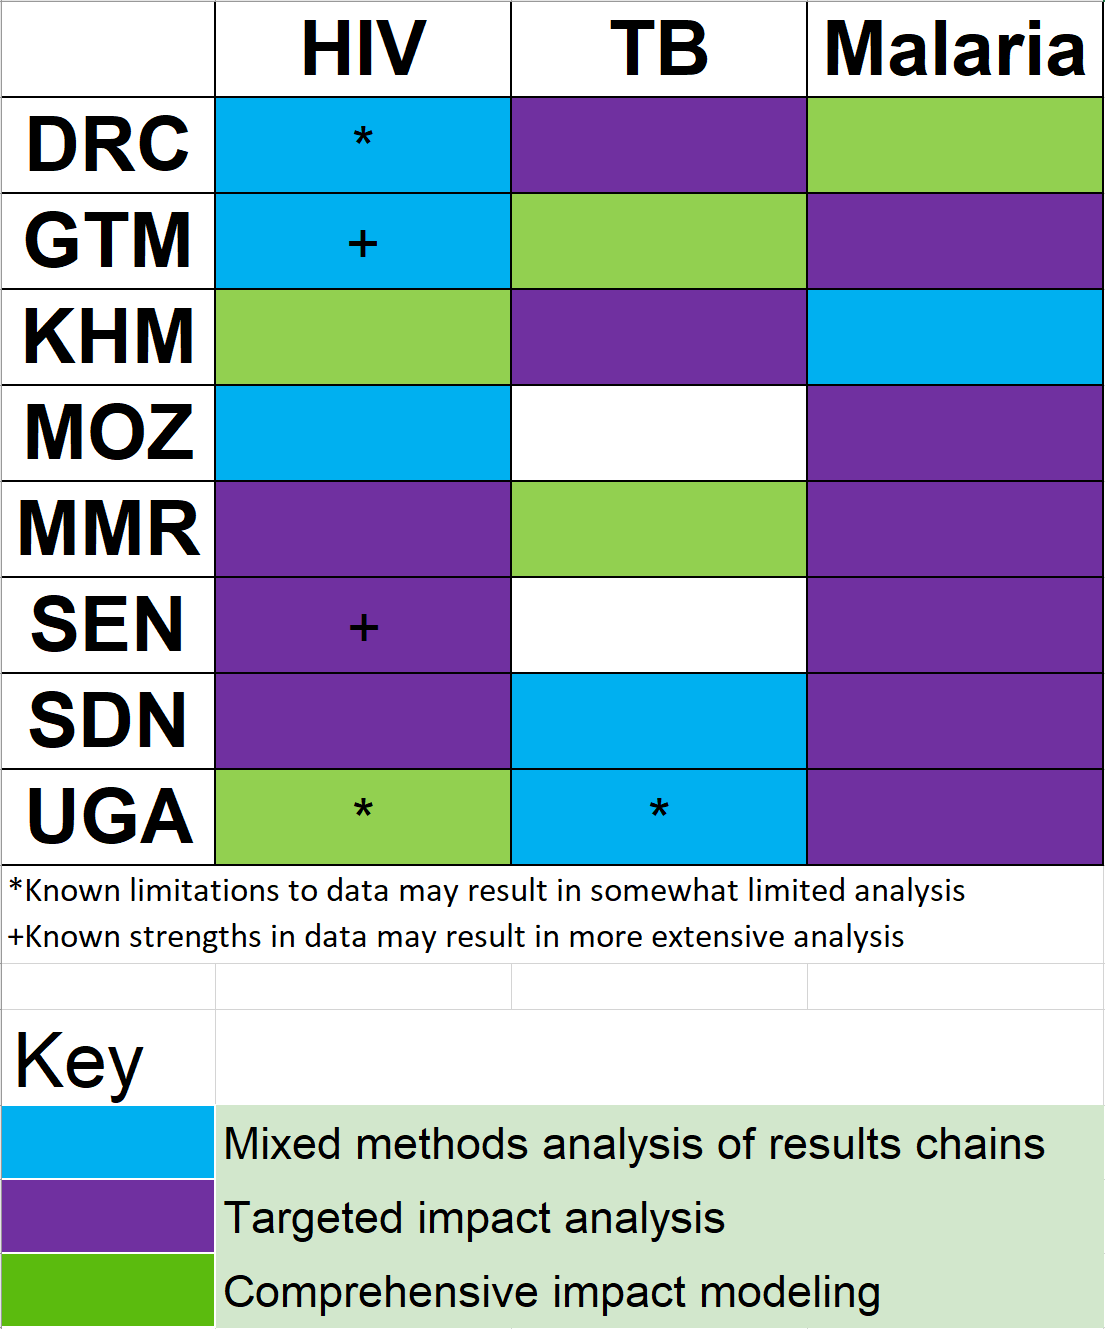
\includegraphics[scale=.4]{Differentiated_Plans_Image.png} \\
  \label{fig1}
\end{figure}


% ------------------------------------------------------------------------------
% Why
\section{Motivation for Differentiated Approaches} \label{why}

There are several reasons why the PCE has opted to take a different approach by disease and country. First and foremost is in an effort to provide results that are relevant to the broad array of audiences who the results might reach. While an overall assessment of the steps leading from Global Fund investment to impact may be relevant and useful to stakeholders in the Global Fund Secretariat, a more tailored analysis focused on isolated sections of the results chains may be more useful to national programs. \\

Second is the feasibility of adding value through impact evaluation. Differences in data availability (indicators tracked and level of disaggregation), data quality, and basic differences in epidemiology limit our ability to apply a generic approach to all diseases in all countries. Furthermore, extensive impact evaluation has already been (or is being) conducted by other organizations for certain diseases in certain countries. For these reasons, the PCE seeks to evaluate different diseases in different ways in order identify applications of existing data that are both possible given known limitations and actually useful to stakeholders. \\

% ------------------------------------------------------------------------------
% Basic Outputs Model
\section{Dose-Response Model}

% Summary
The idea behind the dose-response model is that greater intensity of investment in one intervention is expected to produce more outputs in its associated indicator and vice-versa. What makes this more complex than a simple comparison of time trends is the fact that each intervention may realistically be expected to produce outputs in multiple indicators, and each activity/output indicator is expected to be impacted by investments in multiple interventions. For example, investment in facility-based treatment of malaria is expected to result in increases in RDTs used and ACTs used (not just one or the other), and so is integrated community case management. Without more detailed data that precisely tracks outputs that are the direct response to certain investments, this sort of many-to-many relationship is necessary to reflect in a model. \\

% the form of the model
Therefore, the central model for measuring the contribution of Global Fund inputs to health systems outputs is a structural equation model which represents the complex relationships between inputs, activities and outputs, and subsequently outputs, outcomes and burden of disease. Figure \ref{fig2} displays an example of what such a model is expected to look like, focusing on the first half of the results chain. \\
\begin{figure}[h]
  \advance\leftskip-.4in
  \caption{\textmd{Example dose-response Model}}
  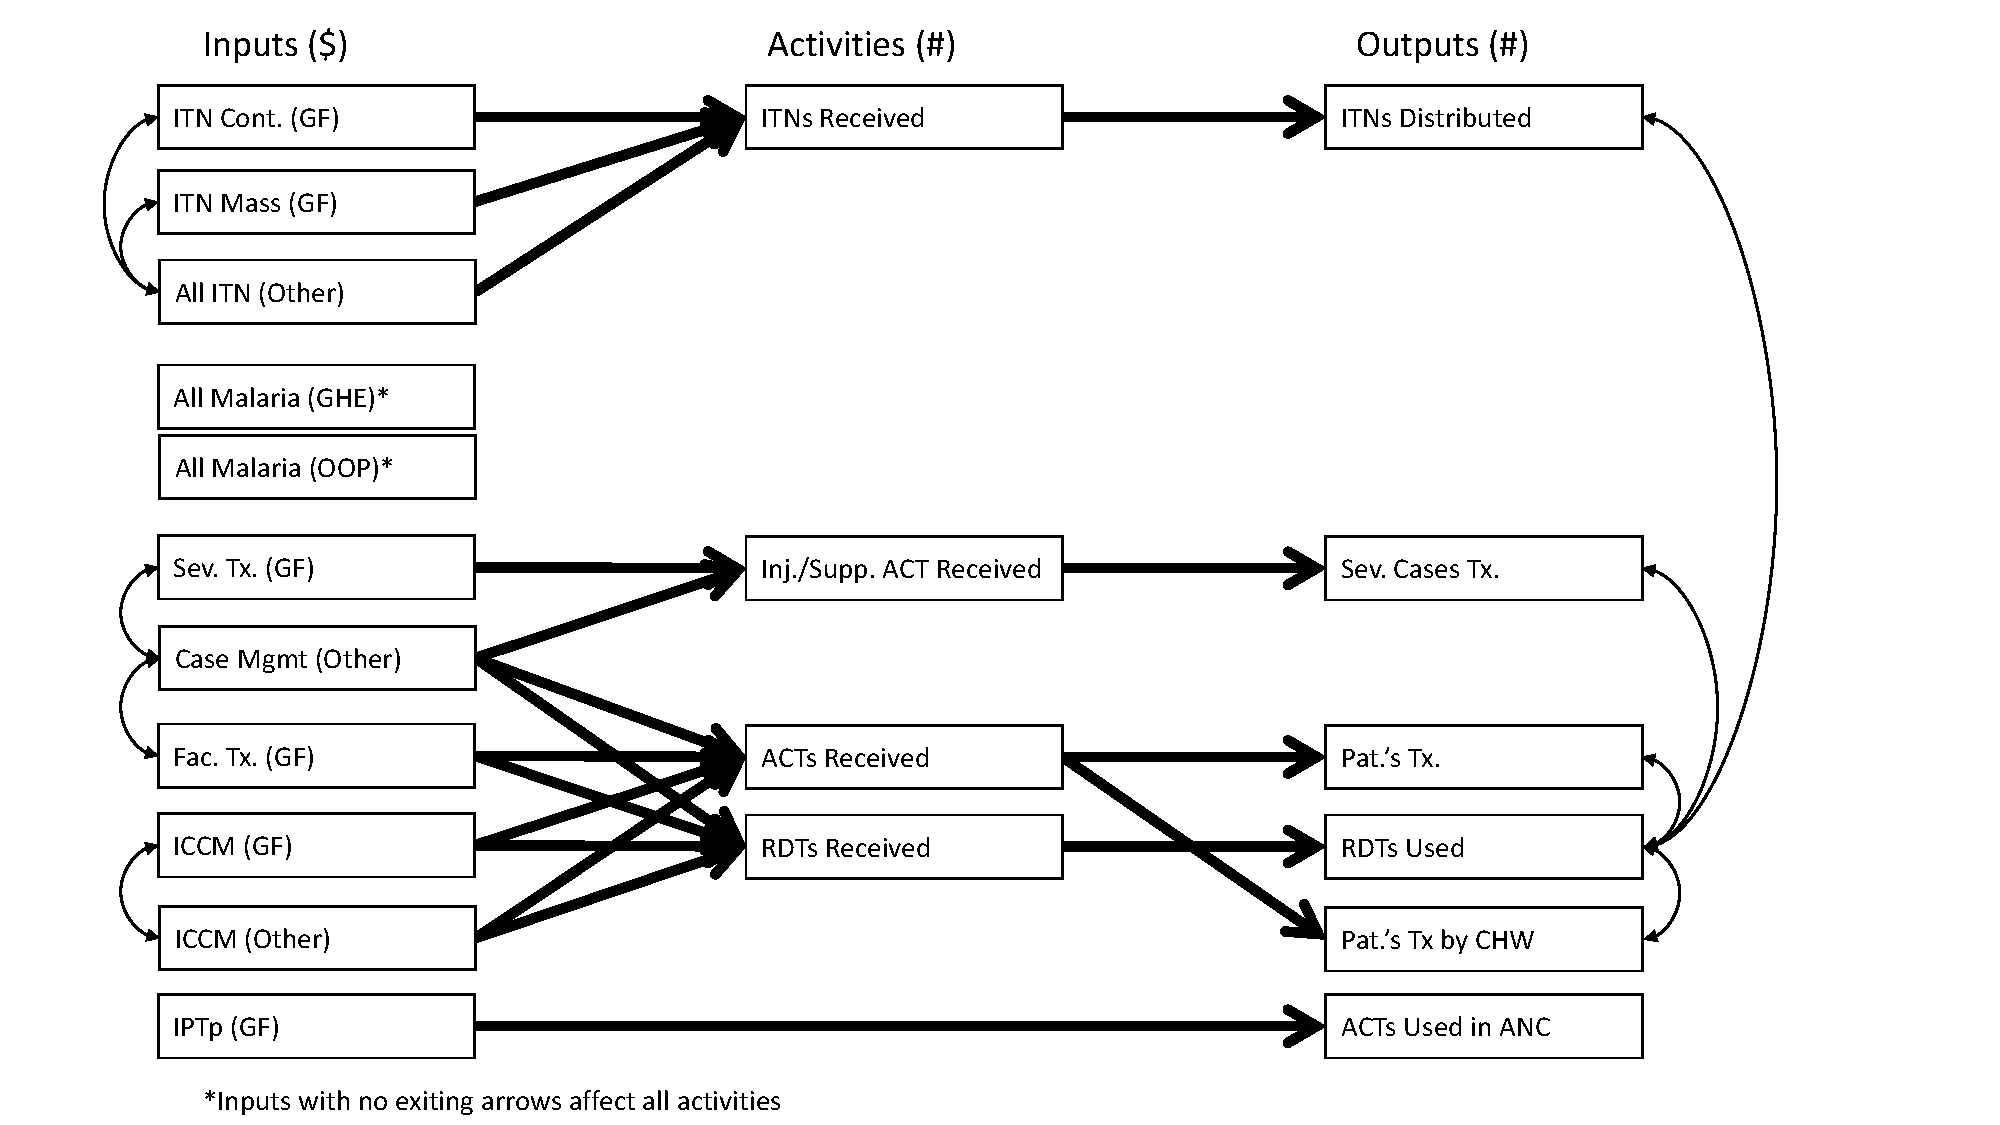
\includegraphics[scale=.35]{SEM_Diagram_Malaria.pdf} \\
  \label{fig2}
\end{figure}

% interpretation
In the figure, each box represents an indicator that is being tracked by the PCE, and the arrows between them represent regression coefficients (i.e. correlations) describing how the indicators co-vary in time. Curved arrows represent correlated error terms, i.e. correlations without an explicit direction. \\

In this way, we can bring together the indicators the PCE is tracking along the results chains and represent their relationships using a structure that accurately reflects their relationships according to our theory of change. For example, this allows us to specify which inputs are intended to impact which outputs, but also which inputs are intended (according to the PCE theory of change) to be allocated in partnership with other donors. A similar model relating indicators between outputs, outcomes and burden of disease will be constructed to represent the second half of the results chain, taking advantage of subnational data as much as possible to find correlations. \\

The PCE is already in the process of measuring these correlations, exemplified in Figure \ref{fig3}. This only displays three of the many interrelated indicators in the full model however, hence the need for a more complex structural equation model. \\

\begin{figure}[h]
  \advance\leftskip-.25in
  \caption{\textmd{Example of Pairwise Correlations as Part of dose-response Model}}
  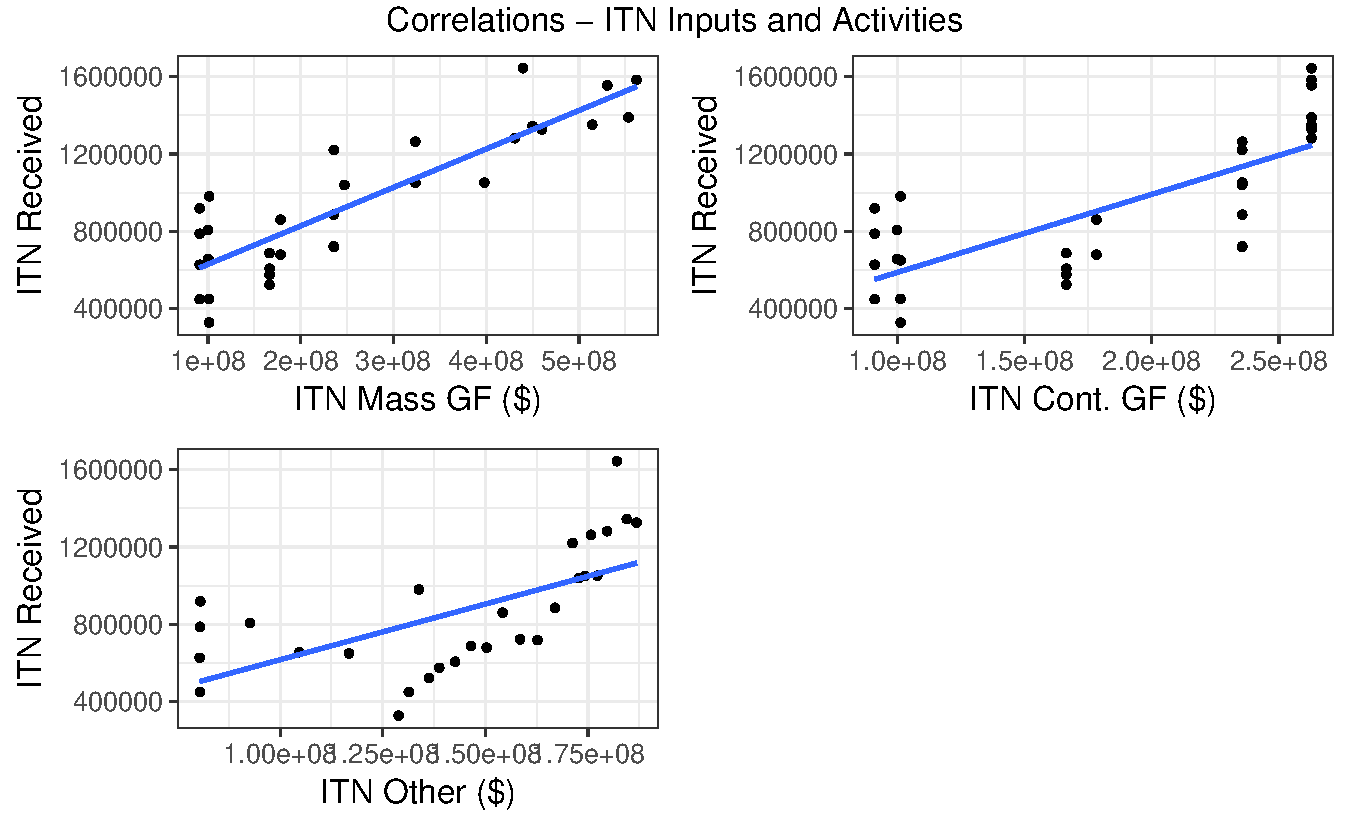
\includegraphics[scale=.375]{Pages_from_pilot_data_exploratory_graphs.pdf} \\
  \label{fig3}
\end{figure}

The final product of dose-response model will focus less on the measurement of coefficients however, and more on the implications of the estimates. We will use counterfactual analysis to describe the anticipated changes in outputs that the model predicts will result from an alternative Global Fund investment. In other words, the PCE will construct a realistic alternative grant budget, and use the model to evaluate the changes in outputs, outcomes and burden of disease that would be expected to result from it. \\

This model relies on several conditions to be reliable. First, the breadth of indicators included in it serves as the most critical constraint to its generalizability. Because most available program data tracks countable commodities, many of the non-commodity interventions may be left out of the model and therefore not reflected in the counterfactual analyses. Second however, including specific control variables will be essential. Indicators of varying data quality, varying unit costs and confounding socio-demographic indicators will be included when possible in order to control for trends that may otherwise explain the relationships between sections of the results chain. \\

% extension to RSSH
\subsection{Extension to RSSH}
In evaluating the contribution of catalytic and system-wide Global Fund investments (such as investments to strengthen resilient and sustainable systems for health (RSSH)), an additional layer of controls may be necessary. This is because such investments are intended to operate in addition to, or synergistically with, other program areas, not to result in outputs on their own. \\

Essentially, this amounts to controlling for spending on RSSH as well as. The dose-response model will be tested with and without the inclusion of RSSH investments and the difference will be assessed in terms of expected outputs and outcomes, as well as total variance in the indicators explained by the model. \\

% ------------------------------------------------------------------------------
% Further Details on Model-Based Geostatistics
\subsection{Relationship with Value for Money} \label{vfm}
The dose-response model has a natural relationship with value for money (VfM) assessment. Focusing on the first half of the results chain, the regression coefficients in the model can be interpreted as cost per output, or efficiency. Focusing on the second half of the results chain, the coefficients can be interpreted as impact per output, or effectiveness. The model will be explored through the lens of VfM in order to explore the relative efficiency and effectiveness of some investments compared to others. \\

\section{Narrative Descriptive Analysis}
The second approach to assessing impact is descriptive analysis of indicators in a sequential fashion along the results chain, with accompanying narrative to explain and contextualize the trends. This approach is now familiar to the PCE and its audiences at time of writing, as it has been presented now in each of the 2018/19 annual country reports and their synthesis. \\

The advantages of this approach are its comprehensiveness. While the dose-response model provides substantial detail about the relationships between variables, it is constrained to those variables which (according to theory) have a corresponding indicator before or after it that can also be measured. Approaching the results chains in a more narrative way enables deeper dives into subpopulations and indicators that may be more isolated quantitatively, but are important nonetheless. \\

\section{Country-Specific Tailored Analyses Based on Context}

The third approach to impact evaluation constitutes the most varied category. Generally speaking, these analyses will focus on a key section of the results chain, specific subnational areas, specific subpopulations or country characteristics that cannot easily be replicated in other countries. Examples of these approaches are still emerging in each country but may include:

\begin{itemize}
  \item Mixed methods analysis of findings arising from the subnational resource tracking study in Uganda. In this context, stakeholders identified a need for understanding financial flows at the district level. The PCE selected five districts to explore in depth to understand how resources are allocated, spent and translating into outputs at the local level. These districts may not be generalizable to the entire country however, so catered analyses will be developed to understand what is happening in these districts alone.
  \item Malaria elimination analysis in Guatemala. Given the epidemiological status of malaria in the Guatemalan context, prevention and community case management activities are focused on very specific hot spots where the parasite is known to remain. Separate modeling approaches are being designed to understand the second half of the results chain in this case specifically.
  \item Rationalization analysis in DRC. In the DRC context, international donors and the government have undergone a process known as rationalization, whereby donors coordinate which geographic areas their investments will be directed towards, and limit their activities elsewhere. This policy offers an unusual opportunity to evaluate donor investment as a ``natural experiment", and analyses may be structured for this situation specifically.
\end{itemize}

These examples are indicative of the types of country-tailored impact evaluations that the PCE is exploring, and may not be the final analyses that the evaluators and stakeholders agree upon. \\

\bibliographystyle{bmc-mathphys} % Style BST file (bmc-mathphys, vancouver, spbasic).
\bibliography{bmc_article}      % Bibliography file (usually '*.bib' )

\end{backmatter}

\end{document}
